\documentclass[tikz,border=5pt]{standalone}
\usepackage[T1]{fontenc}
\usepackage{lmodern,amsmath,amssymb}
\usetikzlibrary{arrows.meta,calc,positioning,fit,backgrounds,shapes.geometric,matrix,decorations.pathreplacing,patterns}
\definecolor{ink}{gray}{0.08}
\definecolor{wash}{gray}{0.965}
\definecolor{soft}{gray}{0.45}
\tikzset{box/.style={draw=ink,line width=.65pt,fill=white,align=center,inner sep=4pt,outer sep=0pt,font=\small},flow/.style={draw=ink,line width=.65pt,-{Latex[length=1.8mm,width=1.3mm]},rounded corners=2pt},annotation/.style={font=\scriptsize,text=soft,align=center},groupbox/.style={draw=soft,dashed,line width=.45pt,fill=wash}}
\begin{document}
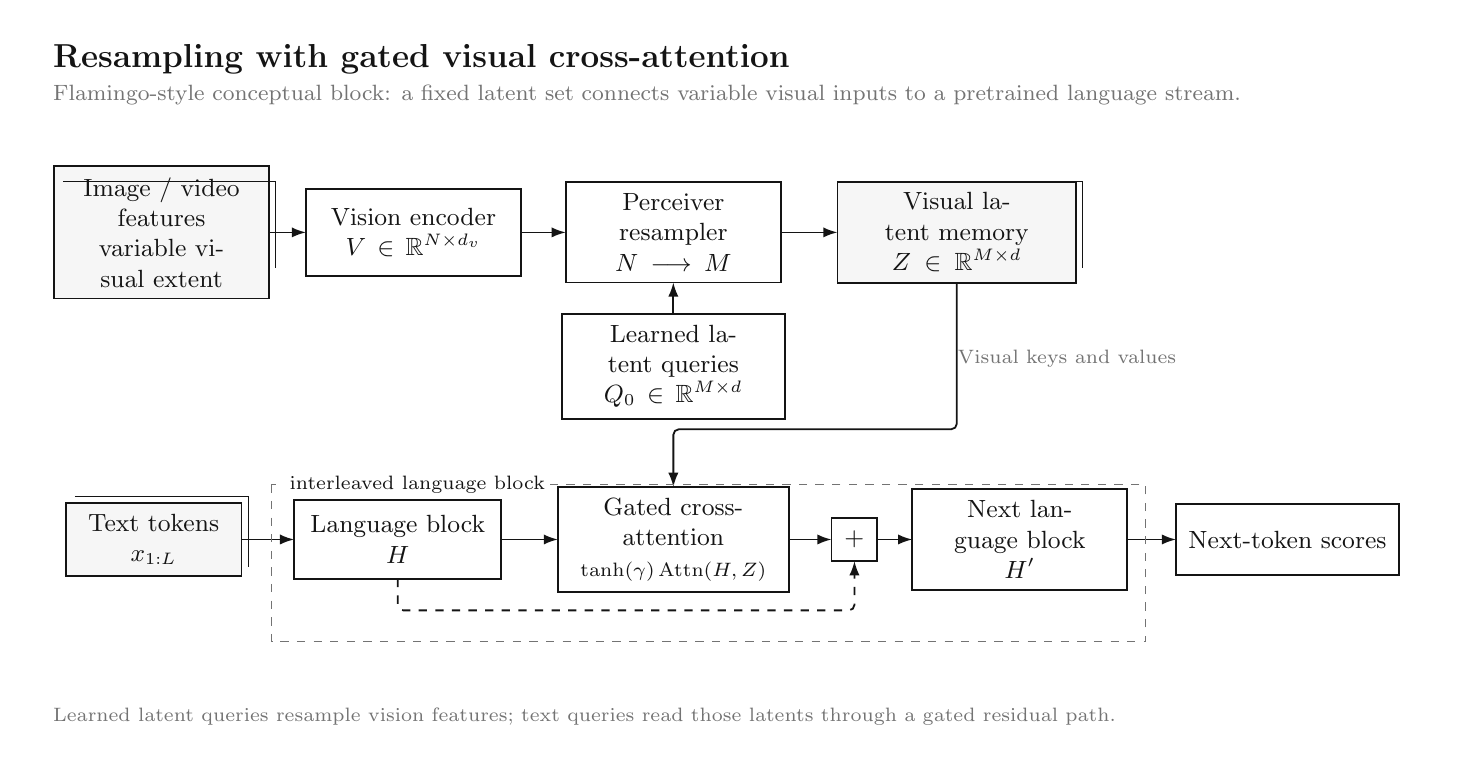
\begin{tikzpicture}[x=1cm,y=-1cm,font=\rmfamily,text=ink]

\path[use as bounding box] (0,0) rectangle (18,9);
\node[anchor=west,font=\large\bfseries] at (.2,.4) {Resampling with gated visual cross-attention};
\node[anchor=west,font=\footnotesize,text=soft] at (.2,.85) {Flamingo-style conceptual block: a fixed latent set connects variable visual inputs to a pretrained language stream.};
\begin{pgfonlayer}{background}
\end{pgfonlayer}
\node[box,fill=wash,minimum width=2.7cm,minimum height=1.1cm,text width=2.45cm] (images) at (1.7,2.6) {Image / video features\\variable visual extent};
\draw[ink,line width=.4pt] (0.44999999999999984,1.9499999999999997) -- (3.15,1.9499999999999997) -- (3.15,3.0500000000000003);
\node[box,minimum width=2.7cm,minimum height=1.1cm,text width=2.45cm] (vision) at (4.9,2.6) {Vision encoder\\$V\in\mathbb{R}^{N\times d_v}$};
\node[box,minimum width=2.7cm,minimum height=1.1cm,text width=2.45cm] (resample) at (8.2,2.6) {Perceiver resampler\\$N\longrightarrow M$};
\node[box,fill=wash,minimum width=3.0cm,minimum height=1.1cm,text width=2.75cm] (latents) at (11.8,2.6) {Visual latent memory\\$Z\in\mathbb{R}^{M\times d}$};
\draw[ink,line width=.4pt] (10.4,1.9499999999999997) -- (13.4,1.9499999999999997) -- (13.4,3.0500000000000003);
\node[box,minimum width=2.8cm,minimum height=0.9cm,text width=2.55cm] (queries) at (8.2,4.3) {Learned latent queries\\$Q_0\in\mathbb{R}^{M\times d}$};
\node[box,fill=wash,minimum width=2.2cm,minimum height=0.9cm,text width=1.9500000000000002cm] (text) at (1.6,6.5) {Text tokens\\$x_{1:L}$};
\draw[ink,line width=.4pt] (0.6,5.95) -- (2.8000000000000003,5.95) -- (2.8000000000000003,6.8500000000000005);
\node[box,minimum width=2.6cm,minimum height=1.0cm,text width=2.35cm] (lm1) at (4.7,6.5) {Language block\\$H$};
\node[box,minimum width=2.9cm,minimum height=1.1cm,text width=2.65cm] (xatt) at (8.2,6.5) {Gated cross-attention\\{\scriptsize $\tanh(\gamma)\,\mathrm{Attn}(H,Z)$}};
\node[box,minimum width=0.55cm,minimum height=0.55cm,text width=0.30000000000000004cm] (sum) at (10.5,6.5) {$+$};
\node[box,minimum width=2.7cm,minimum height=1.0cm,text width=2.45cm] (lm2) at (12.6,6.5) {Next language block\\$H^{\prime}$};
\node[box,minimum width=2.8cm,minimum height=0.9cm,text width=2.55cm] (out) at (16.0,6.5) {Next-token scores};
\begin{pgfonlayer}{background}
\draw[flow] (images.east) -- (vision.west);
\draw[flow] (vision.east) -- (resample.west);
\draw[flow] (resample.east) -- (latents.west);
\draw[flow] (queries.north) -- (resample.south);
\draw[flow] (text.east) -- (lm1.west);
\draw[flow] (lm1.east) -- (xatt.west);
\draw[flow] (xatt.east) -- (sum.west);
\draw[flow] (sum.east) -- (lm2.west);
\draw[flow] (lm2.east) -- (out.west);
\draw[flow] (latents.south) -- (11.8,5.1) -- (8.2,5.1) -- (xatt.north);
\draw[flow,dashed] (lm1.south) -- (4.7,7.4) -- (10.5,7.4) -- (sum.south);
\end{pgfonlayer}
\draw[draw=soft,dashed,line width=.45pt] (3.1,5.8) rectangle (14.2,7.8);
\node[anchor=west,font=\scriptsize,fill=white,inner sep=2pt] at (3.25,5.8) {interleaved language block};
\node[annotation,text width=3.0cm] at (13.2,4.2) {Visual keys and values};
\node[anchor=west,align=left,font=\scriptsize,text=soft,text width=17.6cm] at (.2,8.75) {Learned latent queries resample vision features; text queries read those latents through a gated residual path.};
\end{tikzpicture}
\end{document}
